\documentclass[aspectratio=169,11pt]{beamer}

\usepackage[T1]{fontenc}
\usepackage[utf8]{inputenc}
\usepackage[ngerman]{babel}
\usepackage{graphicx}
\usepackage{booktabs}
\usepackage{tikz}
\usepackage{tcolorbox}
\usetikzlibrary{arrows.meta,positioning,fit,backgrounds}

\definecolor{ink}{HTML}{101820}
\definecolor{panel}{HTML}{F5F7FA}
\definecolor{linegray}{HTML}{D9E0E8}
\definecolor{muted}{HTML}{64748B}
\definecolor{accent}{HTML}{00A6A6}
\definecolor{accenttwo}{HTML}{FFB000}
\definecolor{deep}{HTML}{17324D}

\setbeamertemplate{navigation symbols}{}
\setbeamertemplate{headline}{}
\setbeamertemplate{blocks}[rounded][shadow=false]
\setbeamercolor{normal text}{fg=ink,bg=white}
\setbeamercolor{frametitle}{fg=ink,bg=white}
\setbeamercolor{title}{fg=white}
\setbeamercolor{subtitle}{fg=linegray}
\setbeamercolor{author}{fg=white}
\setbeamercolor{institute}{fg=linegray}
\setbeamercolor{date}{fg=linegray}
\setbeamercolor{block title}{fg=white,bg=deep}
\setbeamercolor{block body}{fg=ink,bg=panel}
\setbeamercolor{itemize item}{fg=accent}
\setbeamercolor{itemize subitem}{fg=accent}
\setbeamerfont{title}{size=\huge,series=\bfseries}
\setbeamerfont{subtitle}{size=\large}
\setbeamerfont{frametitle}{size=\Large,series=\bfseries}
\setbeamerfont{block title}{series=\bfseries}
\setbeamersize{text margin left=0.75cm,text margin right=0.75cm}

\setbeamertemplate{itemize item}{\raise0.15ex\hbox{\scriptsize$\blacktriangleright$}}
\setbeamertemplate{itemize subitem}{\raise0.15ex\hbox{\tiny$\blacktriangleright$}}
\setbeamertemplate{frametitle}{
  \vspace{0.1cm}
  \begin{beamercolorbox}[wd=\paperwidth,ht=0.95cm,leftskip=0.72cm,rightskip=0.72cm]{frametitle}
    \usebeamerfont{frametitle}\insertframetitle
    \hfill
    \tikz[baseline=-0.6ex]\fill[accent] (0,0) circle (2.2pt);
  \end{beamercolorbox}
  \vspace{-0.25cm}
  \begin{tikzpicture}[remember picture,overlay]
    \draw[linegray,line width=0.45pt]
      ([xshift=0.72cm,yshift=-1.04cm]current page.north west) --
      ([xshift=-0.72cm,yshift=-1.04cm]current page.north east);
  \end{tikzpicture}
  \vspace{0.15cm}
}
\setbeamertemplate{footline}{
  \begin{tikzpicture}[remember picture,overlay]
    \fill[linegray] (current page.south west) rectangle ([yshift=1.6pt]current page.south east);
    \fill[accent] (current page.south west) rectangle
      ([xshift={\paperwidth*\insertframenumber/\inserttotalframenumber},yshift=1.6pt]current page.south west);
    \node[anchor=south east, text=muted, font=\scriptsize] at ([xshift=-0.35cm,yshift=0.12cm]current page.south east)
      {\insertframenumber/\inserttotalframenumber};
  \end{tikzpicture}
}

\newtcolorbox{modernbox}[1]{
  colback=panel,
  colframe=accent,
  coltitle=ink,
  fonttitle=\bfseries,
  title=#1,
  arc=1.5mm,
  boxrule=0.7pt,
  left=2.5mm,
  right=2.5mm,
  top=1.5mm,
  bottom=1.5mm
}

\title{Raspberry Pi Robotik Controller}
\subtitle{Zweiteilige Projektarbeitspr\"asentation}
\author{Christoph Hackl \and Moritz Klein}
\institute{HTBLuVA St. P\"olten -- 4AHELS}
\date{Schuljahr 2025/2026}

\newcommand{\smallitem}{\setlength{\itemsep}{0.45em}}

\begin{document}

\begin{frame}[plain]
  \begin{tikzpicture}[remember picture,overlay]
    \fill[ink] (current page.south west) rectangle (current page.north east);
    \fill[accent] (current page.south west) rectangle ([xshift=0.18\paperwidth]current page.north west);
    \node[anchor=east, opacity=0.28] at ([xshift=1.0cm,yshift=-0.25cm]current page.east)
      {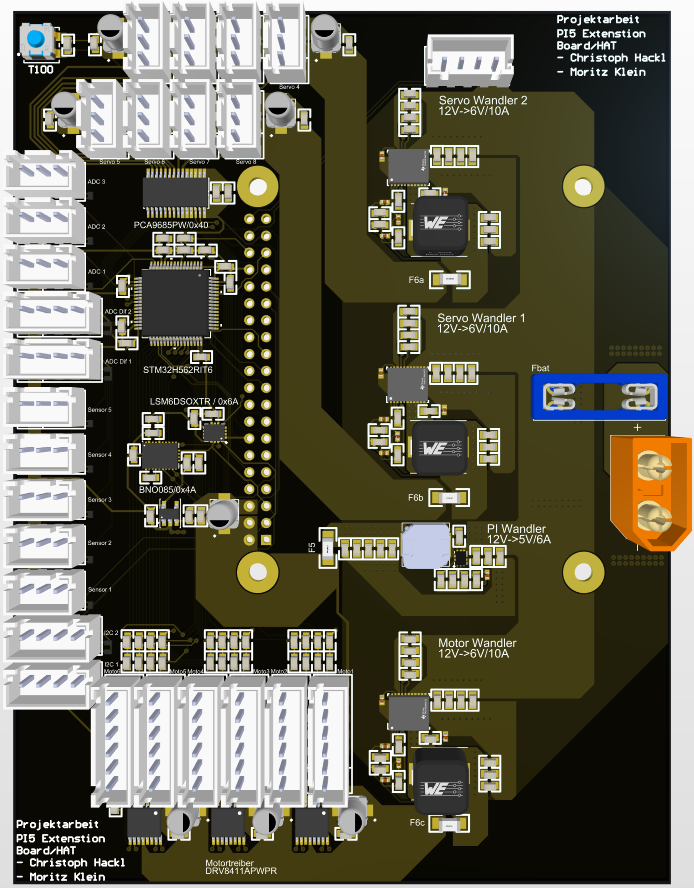
\includegraphics[height=0.86\paperheight]{img/Board.png}};
    \node[anchor=west, align=left, text=white] at ([xshift=0.95cm,yshift=0.9cm]current page.west) {
      {\usebeamerfont{title}\inserttitle}\\[0.35cm]
      {\usebeamerfont{subtitle}\color{linegray}\insertsubtitle}\\[1.0cm]
      {\large Christoph Hackl \quad|\quad Moritz Klein}\\[0.2cm]
      {\color{linegray}HTBLuVA St. P\"olten -- 4AHELS}
    };
    \node[anchor=south west, text=linegray, font=\small] at ([xshift=0.95cm,yshift=0.5cm]current page.south west)
      {Schuljahr 2025/2026};
  \end{tikzpicture}
\end{frame}

\begin{frame}{Projektziel}
  \begin{columns}[T,onlytextwidth]
    \column{0.55\textwidth}
      \begin{itemize}
        \smallitem
        \item Erweiterungsplatine f\"ur den Raspberry Pi 5
        \item Motoren, Servos, Sensoren und Versorgung auf einem Board
        \item Einsatz im ECER-Robotik-Wettbewerb und f\"ur Schulprojekte
        \item Robuster Aufbau statt vieler einzelner Zusatzmodule
      \end{itemize}
    \column{0.40\textwidth}
      \begin{block}{Kernidee}
        Raspberry Pi f\"ur Hauptlogik, Bildverarbeitung und Entscheidungen.
        STM32 f\"ur zeitkritische Signale, ADC und Motoransteuerung.
      \end{block}
  \end{columns}
\end{frame}

\begin{frame}{Systemarchitektur}
  \centering
  \begin{tikzpicture}[
    scale=0.82,
    transform shape,
    font=\small,
    block/.style={draw, rounded corners=2pt, minimum width=2.7cm, minimum height=0.9cm, align=center, fill=blue!10},
    io/.style={draw, rounded corners=2pt, minimum width=2.4cm, minimum height=0.8cm, align=center, fill=green!10},
    line/.style={-{Latex[length=2mm]}, thick}
  ]
    \node[block] (rpi) {Raspberry Pi 5\\Main Control};
    \node[block, right=2.4cm of rpi] (stm) {STM32H562\\Realtime / ADC};
    \node[block, right=2.2cm of stm] (drv) {DRV8411\\Motortreiber};
    \node[io, below=1.2cm of drv] (mot) {DC-Motoren\\Encoder};
    \node[block, below=1.2cm of rpi] (pca) {PCA9685\\Servo-PWM};
    \node[io, left=1.5cm of pca] (servo) {Servos};
    \node[io, above=1.1cm of rpi] (imu) {IMUs / digitale\\Sensorik};
    \node[io, above=1.1cm of stm] (ana) {Analoge\\Sensorik};
    \node[io, above=1.1cm of drv] (power) {Powerrails\\12 V auf 6 V / 5 V / 3,3 V};

    \draw[line] (rpi) -- node[above] {UART} (stm);
    \draw[line] (stm) -- node[above] {PWM} (drv);
    \draw[line] (drv) -- (mot);
    \draw[line] (mot) -- node[below] {Encoder} (stm);
    \draw[line] (rpi) -- node[right] {I\textsuperscript{2}C} (pca);
    \draw[line] (pca) -- (servo);
    \draw[line] (imu) -- (rpi);
    \draw[line] (ana) -- (stm);
    \draw[line] (power) -- (drv);
    \draw[line] (power) -- (stm);
    \draw[line] (power) -- (rpi);
  \end{tikzpicture}
\end{frame}

\section{Teil 1: Christoph Hackl}

\begin{frame}{Christoph: Aufgabenbereich}
  \begin{columns}[T,onlytextwidth]
    \column{0.52\textwidth}
      \begin{itemize}
        \smallitem
        \item Motorsteuerung und Motoranschl\"usse
        \item Servosteuerung \"uber PCA9685
        \item Sensoranbindungen und Testpunkte
        \item Schutzbeschaltungen und Debug-M\"oglichkeiten
      \end{itemize}
    \column{0.42\textwidth}
      \begin{itemize}
        \smallitem
        \item Encoder-Auswertung
        \item Sensor-Softwareintegration
        \item Funktionspr\"ufung von Aktoren und Sensorsignalen
      \end{itemize}
  \end{columns}
\end{frame}

\begin{frame}{Motoren, Servos und Sensorik}
  \begin{columns}[T,onlytextwidth]
    \column{0.53\textwidth}
      \begin{itemize}
        \smallitem
        \item Drei DRV8411-Treiber f\"ur DC-Motoren
        \item PWM-Erzeugung durch den STM32
        \item Encoder-R\"uckmeldung f\"ur sp\"atere Regelung
        \item Servos \"uber getrennten Versorgungsbereich
        \item Analoge Sensorik am STM32, digitale Sensorik am Pi
      \end{itemize}
    \column{0.42\textwidth}
      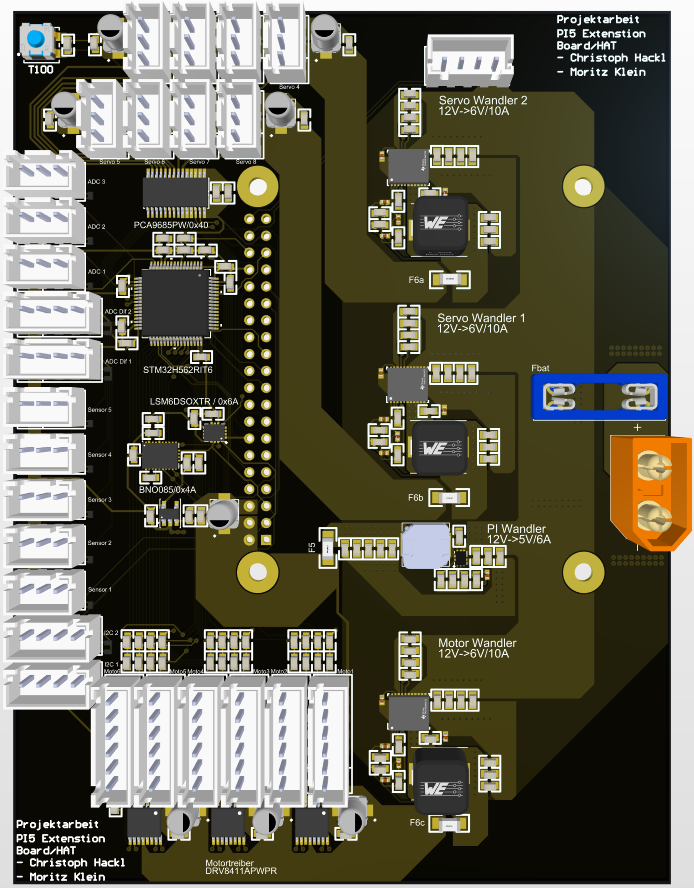
\includegraphics[width=\linewidth,height=0.62\textheight,keepaspectratio]{img/Board.png}
  \end{columns}
\end{frame}

\begin{frame}{STM32-Firmware f\"ur Aktoren}
  \begin{itemize}
    \smallitem
    \item Grundkonfiguration in STM32CubeIDE angelegt
    \item PWM-Kan\"ale f\"ur Motoren werden nach dem Start initialisiert
    \item UART-Kommandos werden in Motorwerte von -100 bis 100 umgesetzt
    \item Encoder-Flanken werden gez\"ahlt und als Statusdaten zur\"uckgemeldet
    \item ADC-Werte werden zusammen mit Encoderwerten periodisch ausgegeben
  \end{itemize}

  \vspace{0.5em}
  \begin{block}{Beispiel f\"ur ein Motor-Kommando}
    \texttt{M 20 -10 0 0 50 -50}
  \end{block}
\end{frame}

\begin{frame}{Messung: Encoder-Signale}
  \begin{columns}[T,onlytextwidth]
    \column{0.48\textwidth}
      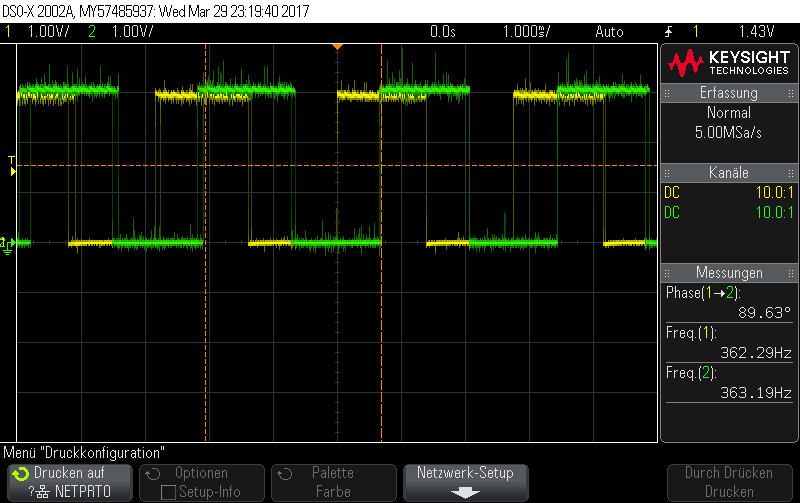
\includegraphics[width=\linewidth]{img/encoder_vorwaerts.png}
      \centering \scriptsize Vorw\"arts: Phasenlage ca. $+90^\circ$
    \column{0.48\textwidth}
      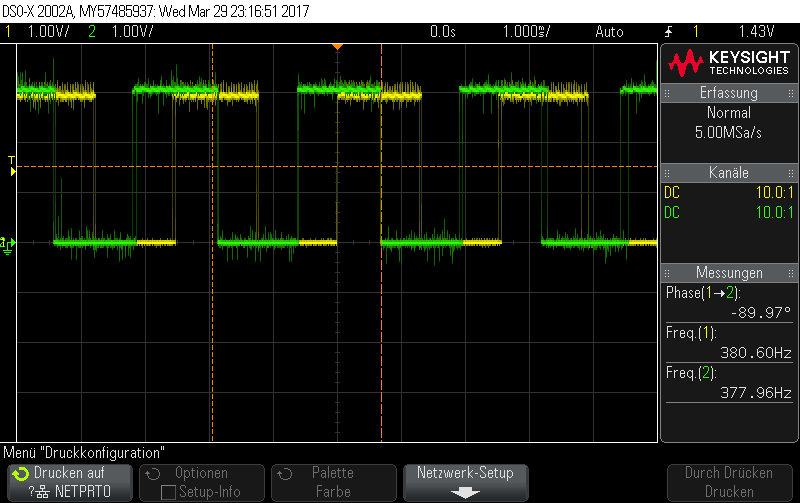
\includegraphics[width=\linewidth]{img/encoder_rueckwaerts.png}
      \centering \scriptsize R\"uckw\"arts: Phasenlage ca. $-90^\circ$
  \end{columns}

  \vspace{0.6em}
  \begin{itemize}
    \item Saubere Quadratur-Signale mit ca. 3 V Pegel
    \item Richtung ist durch Vorzeichen der Phasenlage erkennbar
    \item Berechnete Drehzahl bei 50\,\% PWM: ca. 93 bis 97 rpm
  \end{itemize}
\end{frame}

\begin{frame}{Christoph: Ergebnis und offene Punkte}
  \begin{columns}[T,onlytextwidth]
    \column{0.49\textwidth}
      \begin{block}{Funktioniert}
        \begin{itemize}
          \item Motortreiber reagieren auf PWM
          \item Encoder liefern plausible Daten
          \item PCA9685 erzeugt Servo-PWM
          \item LSM6DSO ist \"uber Software erreichbar
        \end{itemize}
      \end{block}
    \column{0.49\textwidth}
      \begin{block}{Offen}
        \begin{itemize}
          \item BNO085 wird aktuell nicht im I\textsuperscript{2}C-Scan gefunden
          \item Vermutlich L\"otproblem oder Leitung am Sensor
          \item Motor-/Servomessungen unter echter Last weiterf\"uhren
        \end{itemize}
      \end{block}
  \end{columns}
\end{frame}

\section{Teil 2: Moritz Klein}

\begin{frame}{Moritz: Aufgabenbereich}
  \begin{columns}[T,onlytextwidth]
    \column{0.52\textwidth}
      \begin{itemize}
        \smallitem
        \item Stromversorgung und Powerrail-Konzept
        \item Akkumanagement und Steckverbindungen
        \item Thermisches Verhalten und Leistungsreserven
        \item Layoutbereiche f\"ur Versorgung und Verkabelung
      \end{itemize}
    \column{0.42\textwidth}
      \begin{itemize}
        \smallitem
        \item Kommunikation zwischen Pi und STM32
        \item Software-Testfunktionen
        \item Messungen an Powerrails und Einschaltverhalten
      \end{itemize}
  \end{columns}
\end{frame}

\begin{frame}{Stromversorgung}
  \begin{itemize}
    \smallitem
    \item 12-V-Eingang passend zu einem 3S1P-Akkusystem
    \item Mehrere 6-V-Schienen f\"ur Motoren und Servos
    \item 5-V-Schiene f\"ur den Raspberry Pi
    \item 3,3-V-Logikversorgung aus der 5-V-Schiene
    \item Trennung von Leistungsteil und Logikbereich gegen St\"oreinfl\"usse
  \end{itemize}

  \vspace{0.4em}
  \begin{block}{Ziel der Auslegung}
    Hohe Lastwechsel von Motoren und Servos sollen die Logikversorgung nicht instabil machen.
  \end{block}
\end{frame}

\begin{frame}{Messung: Powerrails unter Last}
  \begin{table}
    \centering
    \small
    \begin{tabular}{lccc}
      \toprule
      Schiene & Leerlauf & Last & Laststrom \\
      \midrule
      6 V Motor & 6,03 V & 5,91 V & 4,12 A \\
      6 V Servo 1 & 6,01 V & 5,94 V & 4,02 A \\
      6 V Servo 2 & 6,08 V & 5,96 V & 4,09 A \\
      5 V Raspberry Pi & 5,02 V & 4,94 V & 1,3 A \\
      \bottomrule
    \end{tabular}
  \end{table}

  \begin{itemize}
    \item Gemeinsame Ausgangsleistung: ca. 79 W
    \item Eingangsleistung bei 12 V und 7,1 A: ca. 85 W
    \item Gesamtwirkungsgrad der Versorgung: ca. 93\,\%
  \end{itemize}
\end{frame}

\begin{frame}{Einschaltverhalten der Motorrail}
  \begin{columns}[T,onlytextwidth]
    \column{0.48\textwidth}
      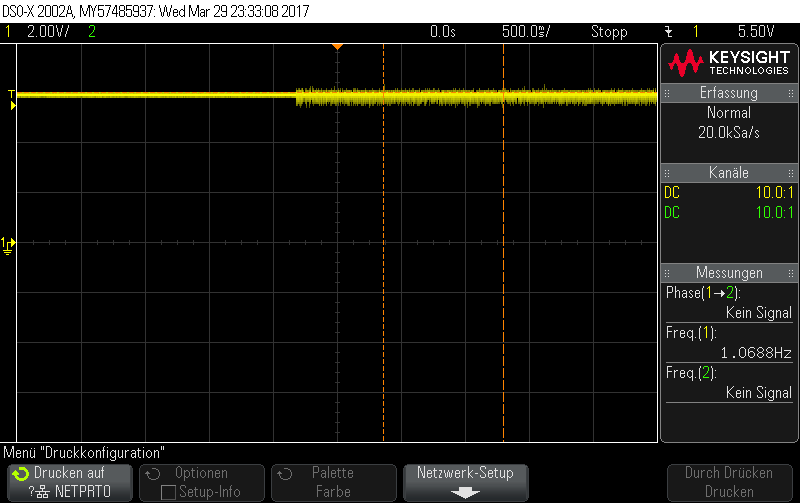
\includegraphics[width=\linewidth]{img/motorrail_einschalten.png}
      \centering \scriptsize Gesamtansicht
    \column{0.48\textwidth}
      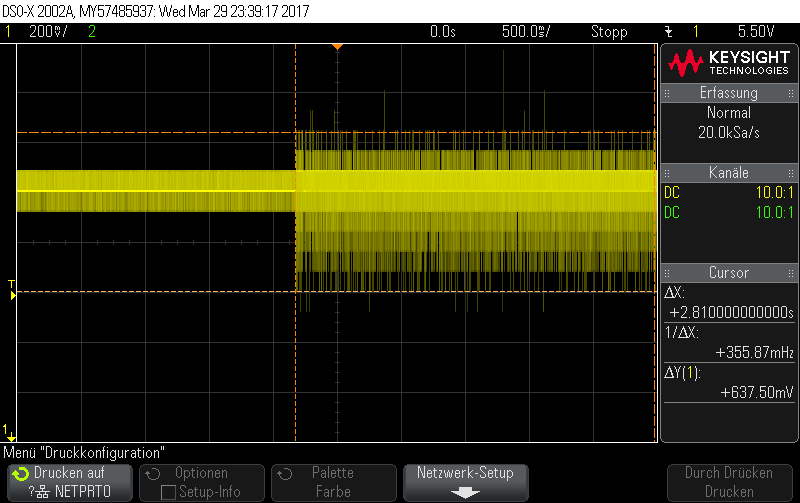
\includegraphics[width=\linewidth]{img/motorrail_zoom.png}
      \centering \scriptsize Zoom im Einschaltmoment
  \end{columns}

  \vspace{0.6em}
  \begin{itemize}
    \item Motorrail steigt grunds\"atzlich funktionsf\"ahig an
    \item Sichtbarer Ripple und kurzer St\"oranteil beim Einschalten
    \item Kein Zusammenbrechen der Versorgung beobachtet
  \end{itemize}
\end{frame}

\begin{frame}{Pi-STM32-Kommunikation}
  \begin{itemize}
    \smallitem
    \item UART mit 115200 Baud, 8 Datenbits, keine Parit\"at, 1 Stoppbit
    \item Kurze ASCII-Kommandos sind f\"ur Steuerwerte und Statusdaten ausreichend
    \item Raspberry Pi sendet Motorbefehle
    \item STM32 sendet Encoder- und ADC-Werte einmal pro Sekunde zur\"uck
  \end{itemize}

  \vspace{0.5em}
  \begin{block}{Beispiel f\"ur eine R\"uckmeldung}
    \texttt{ENC 120 118 0 0 -34 -31 ADC 2048 2011 1995 1020 980}
  \end{block}
\end{frame}

\begin{frame}{Moritz: Ergebnis und Verbesserungen}
  \begin{columns}[T,onlytextwidth]
    \column{0.49\textwidth}
      \begin{block}{Funktioniert}
        \begin{itemize}
          \item 6-V-, 5-V- und 3,3-V-Versorgung funktionieren
          \item Powerrails bleiben unter Last stabil
          \item UART-Kommandos werden verarbeitet
          \item SWD-Programmierung des STM32 funktioniert
        \end{itemize}
      \end{block}
    \column{0.49\textwidth}
      \begin{block}{Verbesserungen}
        \begin{itemize}
          \item Schutz f\"ur 5-V-Wandler beim Akku-Abziehen
          \item Feedback-Netzwerk mechanisch besser sch\"utzen
          \item Reset-Pullup wurde nachtr\"aglich erg\"anzt
        \end{itemize}
      \end{block}
  \end{columns}
\end{frame}

\begin{frame}{Fazit}
  \begin{itemize}
    \smallitem
    \item Das Grundkonzept der Hardwareplattform funktioniert.
    \item Motoren, Servos, Sensorik, Stromversorgung und Kommunikation sind auf einer Platine zusammengef\"uhrt.
    \item Die Messungen zeigen stabile Powerrails und plausible Encoder-Signale.
    \item Offene Punkte liegen vor allem bei BNO085, Schutzma{\ss}nahmen und weiteren Lasttests.
  \end{itemize}

  \vspace{0.7em}
  \begin{center}
    \Large Fragen?
  \end{center}
\end{frame}

\end{document}
